% Cover letter: Product Manager (Prototyping/Design Specialization), N-iX
% CV: Sections/cv_pm_prototyping.tex -> cv_gen/cv_giovanni_tauro-n_ix.pdf
\documentclass[11pt,a4paper,sans]{moderncv}
% Shared preamble and header for the cover letters.
% One main file per application: cl_<company>.tex, built to
% cv_gen/coverletter_giovanni_tauro-<company>.pdf next to cv_giovanni_tauro-<company>.pdf.
% Paths (cl_gen/..., Pictures/...) are relative to the project root, as in the CV (see .latexmkrc).

\moderncvstyle{classic}
\moderncvcolor{blue}

\usepackage[scale=0.80]{geometry}
\setlength{\footskip}{136.00005pt}

\usepackage{fontawesome5}
% hyperref is loaded by moderncv itself; loading it here causes an option clash
\usepackage{xcolor}
\usepackage{graphicx}
\ifxetexorluatex
  \usepackage{fontspec}
  \usepackage{unicode-math}
  \defaultfontfeatures{Ligatures=TeX}
  \setmainfont{Latin Modern Roman}
  \setsansfont{Latin Modern Sans}
  \setmonofont{Latin Modern Mono}
  \setmathfont{Latin Modern Math}
\else
  \usepackage[T1]{fontenc}
  \usepackage{lmodern}
\fi

\usepackage[english]{babel}

% used for the PDF title and the letter closing; the visible header is \clheader below
\name{Giovanni}{Tauro}

% Header: #1 = headline under the name (same as the headline of the matching CV)
\newcommand{\clheader}[1]{%
\noindent
\begin{minipage}[c]{0.74\textwidth}
    {\Huge \textbf{Giovanni Tauro}}\\[-0.2em]
    {\small #1}\\[0.3em]

    \footnotesize
    \faMapMarker*~
    \href{https://www.google.com/maps/search/?api=1&query=Lecco+23900+Italy}
    {\color{blue}Bari-Lecco, Italy}
    \quad
    \faPhone*~
    \href{https://wa.me/393279437161}
    {\color{blue}+39 3279437161}
    \quad
    \faEnvelope~
    \href{mailto:giovanni.taurodi@gmail.com}
    {\color{blue}giovanni.taurodi@gmail.com}
    \\[-0.1em]

    \faLinkedin~
    \href{https://www.linkedin.com/in/giovanni-tauro-gt/}
    {\color{blue}LinkedIn}
    \quad
    \faGithub~
    \href{https://github.com/jotades}
    {\color{blue}GitHub}
    \quad
    \faGraduationCap~
    \href{https://scholar.google.com/citations?user=BS0aVGgAAAAJ&hl=it}
    {\color{blue}Scholar}
    \quad
    \faFilePdf~
    \href{https://www.notion.so/Giovanni-Tauro-2a7901d92f3a800b892af425c5875c6a}
    {\color{blue}Portfolio}
    \quad
    \faCubes~
    \href{https://grabcad.com/giovanni.tauro-3}
    {\color{blue}GrabCAD}

\end{minipage}
\hfill
\begin{minipage}[c]{0.18\textwidth}
    \raggedleft
    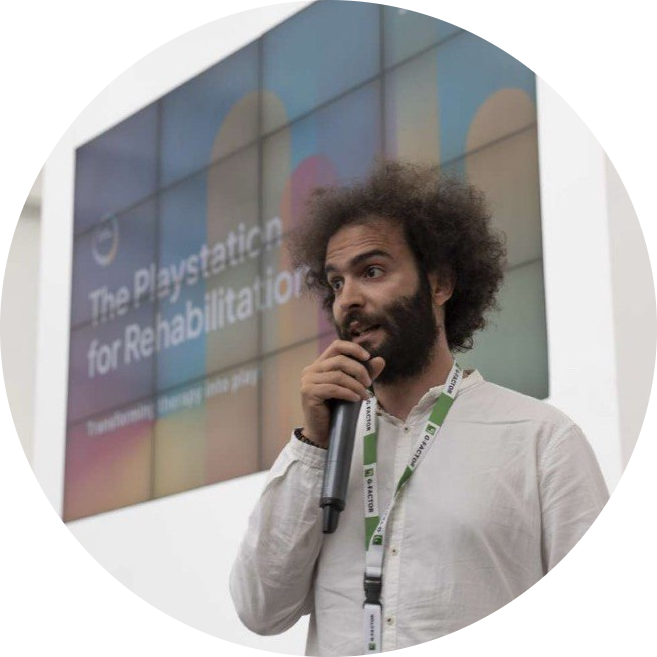
\includegraphics[width=2.8cm]{Pictures/Giovanni_pitch}
\end{minipage}
\vspace{0.1em}
}

\makeatletter
% the sender details are already in \clheader, so skip moderncv's own block
\@detailsfalse
% closing phrase, signature, name
\renewcommand*{\makeletterclosing}{%
  \@closing\\[0.6em]%
  
\includegraphics[height=1.2cm]{Pictures/sign_gt.jpg}\\[0.2em]%
  {\bfseries\@firstname~\@lastname}}
\makeatother


\begin{document}

\clheader{Head of Product | Discovery, UX \& Rapid Prototyping}

\recipient{Product Management Office}{N-iX}
\opening{Dear Hiring Team,}
\closing{Sincerely,}
\makelettertitle

I am applying for the Product Manager role with the Prototyping/Design specialization. I am Head of Product and co-founder of Rehabilia Technologies, and for more than five years I have designed and prototyped products at CNR-STIIMA, the Italian National Research Council. Your description of the role, helping someone decide with a tangible prototype whether an idea deserves investment, is close to how I already work.

At Rehabilia I own the product from discovery to delivery. I interview clinicians, patients and partners, frame the problem, write the requirements and decide what goes into a prototype, an MVP or a later iteration, with a milestone-based roadmap that research partners and funders can follow. Our device, PhiCube, reached a usability score of 85.8/100 (SUS) with 19 children and is now in two ongoing multicentre studies with 134 patients. Presenting it to clinicians, partners and the EIT Health bootcamps taught me to explain the value of a plan to people with very different priorities.

I match the prototype to the question it has to answer. Sometimes that is a flow in Figma, sometimes a coded prototype built with AI assistance: I use Claude and Claude Code in my daily work and hold Anthropic's certifications for both. When the question is physical, it is working hardware: at an LMU Munich challenge my team went from idea to a working rehabilitation proof of concept in 24 hours. At CNR-STIIMA I have taken more than three functional prototypes from concept to experimental validation, and I often map system states and interactions in diagrams so that clinical and research teams can discuss a complex system.

Most of my sessions so far have been with clinicians, researchers and partners rather than consultancy clients, and I have not yet worked in a pre-sales setting. What I bring is the habit of running these conversations with people outside my field, challenging assumptions politely and agreeing on what to test first. My portfolio is linked above.

I would welcome the chance to discuss the role further.

\makeletterclosing

\end{document}
